\documentclass[tikz,border=10pt]{standalone}
\usepackage{pgfplots}
\pgfplotsset{compat=1.18}
\usepackage{amsmath,amssymb,bm}
\definecolor{darkbg}{HTML}{1a1a1a}
\definecolor{lightfg}{HTML}{e8e6e3}
\definecolor{accent}{HTML}{7cb87c}
\definecolor{accent2}{HTML}{6aa0b0}
\definecolor{mutedcol}{HTML}{9a9a9a}
\definecolor{bordercol}{HTML}{3d3d3d}
\definecolor{redcol}{HTML}{cc3333}
\definecolor{bluecol}{HTML}{4466cc}
\pagecolor{darkbg}
\color{lightfg}

\usetikzlibrary{arrows.meta}

\begin{document}
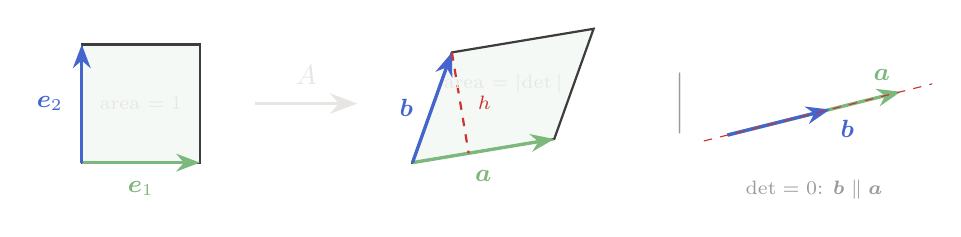
\begin{tikzpicture}

% === PART 1: Unit square ===
\begin{scope}[shift={(0,0)}]
  \fill[accent, opacity=0.08] (0,0) rectangle (1.5,1.5);
  \draw[bordercol, thick] (0,0) rectangle (1.5,1.5);

  \draw[-{Stealth[length=3mm]}, accent, very thick]
    (0,0) -- (1.5,0) node[midway, below=3pt, accent, font=\small] {$\bm{e}_1$};
  \draw[-{Stealth[length=3mm]}, bluecol, very thick]
    (0,0) -- (0,1.5) node[midway, left=3pt, bluecol, font=\small] {$\bm{e}_2$};

  \node[lightfg, font=\scriptsize] at (0.75,0.75) {area $= 1$};
\end{scope}

% === Arrow A ===
\draw[-{Stealth[length=3.5mm]}, lightfg, very thick]
  (2.2,0.75) -- (3.5,0.75)
  node[midway, above=3pt, lightfg, font=\normalsize] {$A$};

% === PART 3: Non-degenerate parallelogram ===
\begin{scope}[shift={(4.2,0)}]
  \pgfmathsetmacro{\ax}{1.8}
  \pgfmathsetmacro{\ay}{0.3}
  \pgfmathsetmacro{\bx}{0.5}
  \pgfmathsetmacro{\by}{1.4}

  \fill[accent, opacity=0.08]
    (0,0) -- (\ax,\ay) -- ({\ax+\bx},{\ay+\by}) -- (\bx,\by) -- cycle;
  \draw[bordercol, thick]
    (0,0) -- (\ax,\ay) -- ({\ax+\bx},{\ay+\by}) -- (\bx,\by) -- cycle;

  \draw[-{Stealth[length=3mm]}, accent, very thick]
    (0,0) -- (\ax,\ay) node[midway, below=3pt, accent, font=\small] {$\bm{a}$};
  \draw[-{Stealth[length=3mm]}, bluecol, very thick]
    (0,0) -- (\bx,\by) node[midway, left=3pt, bluecol, font=\small] {$\bm{b}$};

  % height h (perpendicular from b tip to a direction)
  \pgfmathsetmacro{\projlen}{(\bx*\ax+\by*\ay)/(\ax*\ax+\ay*\ay)}
  \pgfmathsetmacro{\footx}{\projlen*\ax}
  \pgfmathsetmacro{\footy}{\projlen*\ay}
  \draw[redcol, dashed, thick] (\bx,\by) -- (\footx,\footy);
  \node[redcol, font=\scriptsize, right] at ({(\bx+\footx)/2+0.1},{(\by+\footy)/2}) {$h$};

  \node[lightfg, font=\scriptsize] at ({(\ax+\bx)/2},{(\ay+\by)/2+0.15})
    {area $= |\!\det|$};
\end{scope}

% === Separator ===
\node[mutedcol, font=\large] at (7.6,0.75) {$\Big|$};

% === PART 4: Degenerate case ===
\begin{scope}[shift={(8.2,0.35)}]
  \draw[-{Stealth[length=3mm]}, accent, very thick]
    (0,0) -- (2.2,0.55) node[above left, accent, font=\small] {$\bm{a}$};
  \draw[-{Stealth[length=3mm]}, bluecol, very thick]
    (0,0) -- (1.3,0.325) node[below right, bluecol, font=\small] {$\bm{b}$};

  \draw[redcol, dashed, thin] (-0.3,-0.075) -- (2.6,0.65);

  \node[mutedcol, font=\scriptsize, anchor=north] at (1.1,-0.45)
    {$\det = 0$: $\bm{b} \parallel \bm{a}$};
\end{scope}

\end{tikzpicture}
\end{document}
